\documentclass[msc,oneside,11pt,norunningheaders]{ubcthesiscpbl}
%[phd,10pt,noupper,runningheaders]{ubcthesis} 
\usepackage[utf8]{inputenc}  
\usepackage{setspace}
\newcommand{\ifdoDoubleSpace}[1]{}
% committee option is for draft: 1.5 spacing
%\makeatletter

\if@twoside
\def\setpageforTOC{\setcounter{page}{2}}
\else
\def\setpageforTOC{}
\fi

\if@twoside
  \def\ps@plain{%
    %\let\@oddfoot\@empty\let\@evenfoot\@empty
    \let\@oddhead\@empty\let\@evenhead\@empty
    %\def\@evenhead{%
    \def\@evenfoot{%
      \parbox{\textwidth}{%
        \makebox[\textwidth]{{\pagenumberfont\thepage}\hfill}
        %\if@headline\vspace{\headlinespace}\fi
        }%
    }%
    %\def\@oddhead{%
    \def\@oddfoot{%
      \parbox{\textwidth}{%
        \makebox[\textwidth]{\hfill{\pagenumberfont\thepage}}
        %\if@headline\vspace{\headlinespace}\fi
      }%
    }%
    }%
\fi

  \def\ps@plain{%
    %\let\@oddfoot\@empty\let\@evenfoot\@empty
    \let\@oddhead\@empty\let\@evenhead\@empty
    %\def\@evenhead{%
    \def\@evenfoot{%
      \parbox{\textwidth}{%
        \makebox[\textwidth]{{\pagenumberfont\thepage}\hfill}
        %\if@headline\vspace{\headlinespace}\fi
        }%
    }%
    %\def\@oddhead{%
    \def\@oddfoot{%
      \parbox{\textwidth}{%
        \makebox[\textwidth]{\hfill{\pagenumberfont\thepage}}
        %\if@headline\vspace{\headlinespace}\fi
      }%
    }%
    }%

\makeatother
\usepackage{phdthesis}
\usepackage{mathptmx} 
\setcounter{secnumdepth}{4}
\setcounter{tocdepth}{4}
\usepackage{varioref} % eqref is in here?????
\usepackage{url} % For a url..
\usepackage{amssymb} % amssymb/amsmath have?? checkmark? eqref?
\usepackage{amsmath} % align environment (everyone says stop using eqnarray!)


\usepackage{index}
% Following two are just black holes to accomodate index calls in the
% variable list table
\newindex{vars}{vidx}{and}{Coded variables}
\newindex{surveyvars}{sidx}{sand}{Survey variables}

\providecommand{\tabularnewline}{\\} % LyX relic

%******** natbib ********************************
% This is a very nice package for bibliographies.  It includes options
% for sorting and compressing bibliographic entries.
%\usepackage[square,authoryear]{natbib} % REMOVED OPTIONS: numbers,sort&compress,
\usepackage[square,comma,numbers,sort&compress]{natbib}

% cPbL: For chapter-level bibliographies:
%\usepackage{bibtopic}
%\bibliographystyle{aguCpbl}%cje}

%******** graphics and graphicx ******************************
% This allows you to include encapsulated postscript files.  If you
% don't have this, comment the \includegraphics{} line following the
% comment "%includegraphics" later in this file.
\usepackage{graphicx}

%******** lscape ******************************
% This allows you to include landscape layout pages by using the
% |landscape| environment. Note that this output might only be valid
% after converting to a postscript or pdf file.
\usepackage{lscape}

%******** psfrag ******************************
% This allows you to replace text in postscript pictures with formated
% latex text.  This allows you to use math in graph labels
% etc. Uncomment the psfrag lines following the "%psfrag" comment
% later in this file if you don't have this package.  The replacements
% will only be visible in the final postscript file: they will be
% listed in the .dvi file but not performed.
\usepackage{psfrag}

%******** afterpage ***************************
% This package allows you to issue commands at the end of the current
% page.  A good use for this is to use the command
% \afterpage{\clearpage} right after a figure.  This will cause the
% figure to be inserted on the page following the current one (or on
% the current page if it will fit) but will not break the page in the
% middle.
\usepackage{afterpage}

%%%%%%%%%%%%%%%%%%%%%%%%%%%%%%%%%%%%%%%%%%%%%%%%%%%%%%%%%%%%%%%%%%%%%%
% Allow a new preface entity which is useful for a DEDICATION
%%%%%%%%%%%%%%%%%%%%%%%%%%%%%%%%%%%%%%%%%%%%%%%%%%%%%%%%%%%%%%%%%%%%%%
% Use as follows:
%     \beforepreface
%     \dedication{To my grandparents ...}
%     \prefacesection{Abstract}   ...
%
% 2000 February 14: cPbL
\def\dedication#1{
  \chapter[Dedication]{} % Put in TOC but don't display "Dedication"
                         % on page
%  \thispagestyle{empty}  % No page number
  \thispagestyle{plain}   % Yes page number
  \vspace{6cm}
  \begin{center}
    #1
  \end{center}
  }
     
% Define a command to start a bib section for manuscript-based thesis
\newcommand{\placeSecBib}[1]{
\forThesis{
\newpage
\begin{btSect}{veblen,evolution,institutions,swb,general,urban,weather,sk} 
\chapter*{Bibliography for #1} 
\addcontentsline{toc}{section}{Bibliography for #1}
\btPrintCited 
\end{btSect} 
\end{btUnit}
}
}

%\renewcommand{\listfigurename}{List of figures}
%\renewcommand{\listtablename}{List of tables}

 
% These commands are optional.  The defaults are shown.
\institution{AGH-University of Science and Technology}
\institutionaddress{Cracow, Poland}
\program{Telecommunications}

% You can issue as many of these as you have...
%\previousdegree{S.B. Physics, Massachusetts Institute of Technology, 1995}
%\previousdegree{M.Sc. Applied Physics, Stanford University, 1998}
%\previousdegree{Ph.D. Applied Physics, Stanford University, 2001}

% These commands are required.
\title{Writing scalable network applications in Python}
\subtitle{}
\author{Łukasz Marcin Dobrzański}
\copyrightyear{2009} 
\submitdate{January 2009}%\today}

\advisor{Andrzej Głowacz}
\advisortitle{Ph.D. in Telecommunications}
% One might want to override the format of the section and chapter
% numbers.  This shows you how to do it.  Note that
\renewcommand\thepart         {\Roman{part}}
\renewcommand\thechapter      {\arabic{chapter}}
\renewcommand\thesection      {\thechapter.\arabic{section}}
\renewcommand\thesubsection   {\thesection.\arabic{subsection}}
\renewcommand\thesubsubsection{\thesubsection.\arabic{subsubsection}}
\renewcommand\theparagraph    {\thesubsubsection.\arabic{paragraph}}
\renewcommand\thesubparagraph {\theparagraph.\arabic{subparagraph}}

\usepackage{relsize}
\newcommand\muchsmaller{\smaller\smaller}
\usepackage{cpblRef}
\usepackage{cpblTables}


% Below is for the data (survey appendix). Gods help me!
\usepackage{psfrag,color,graphicx}
\graphicspath{{/home/cpbl/papers/incomeCMA/plots/}{./}}

\graphicspath{{/home/cpbl/models/veblenNeighbourhoods/figuresLEL/}{/home/cpbl/models/veblenNeighbourhoods/figuresvs/}{./}{./figuresvs}{./tmpg}{/home/cpbl/papers/incomeCMA/plots/}{./}}
\usepackage{amsthm}
\usepackage{ushort} % For an underbar that looks like \bar.
\usepackage{wrapfig} % For acknowledgements only

% BELOW DEFINES THE THEOREM ENVIROS I NEED: PROPOSITION, LEMMA, PROOF
\newtheorem{theorem}{Theorem}[section]
\newtheorem{lemma}[theorem]{Lemma}
\newtheorem{proposition}[theorem]{Proposition}
\newtheorem{corollary}[theorem]{Corollary}

\newenvironment{definition}[1][Definition]{\begin{trivlist}
\item[\hskip \labelsep {\bfseries #1}]}{\end{trivlist}}
\newenvironment{example}[1][Example]{\begin{trivlist}
\item[\hskip \labelsep {\bfseries #1}]}{\end{trivlist}}
\newenvironment{remark}[1][Remark]{\begin{trivlist}
\item[\hskip \labelsep {\bfseries #1}]}{\end{trivlist}}

% Some tools to differentiate between thesis version and journal
% manuscript version.
\newcommand{\forThesis}[1]{#1}
\newcommand{\forPaper}[1]{}



\newcommand{\LELcfig}[1]{\includegraphics[width=0.75\textwidth,keepaspectratio]{#1.\epspdf}}%{\input{#1}.tex}
% Above redundant: see cpblRef.sty LELwfig

\newcommand{\epspdf}{pdf}%{eps}%
\newcommand{\cmykrgb}{cmyk}%{rgb}
\newcommand{\rawplotspath}{/home/cpbl/models/veblenNeighbourhoods/plots/raw/}
\newcommand{\iCMArawplotspath}{/home/cpbl/econ/favouritePlots/cityScatterPlots/}%{papers/incomeCMA/plots/raw/}
\usepackage[footnotesize,bf]{caption} % Does this actually call caption2 or caption3?
\setlength{\captionmargin}{20pt}


% Inconspicuous hyperref -- very nice.
  \usepackage[   
       colorlinks,
      citecolor=black,
       filecolor=black,
       linkcolor=black,
       urlcolor=black  
   ]{hyperref}

\newif\ifNBER

%%% TURN OFF COMMENTS:
\renewcommand{\draftComment}[1]{}
\renewcommand{\safeDraftComment}[1]{}
\renewcommand{\cpblOldComment}[1]{}

% Turn on comments:

%\renewcommand{\draftComment}{\draftCommentColouredBox}
%\renewcommand{\cpblOldComment}{\draftCommentColouredBox}
 
% UBC has strange format requirements, but some things not strict. So
% don't worry about things looking nice. Widen so I can fit my big tables:
% To ensure that the margin fiddling for the huge/wide/long tables
%\addtolength\oddsidemargin{-1cm}
%\addtolength\evensidemargin{-1cm}
%\addtolength\textwidth{2cm}
\addtolength\oddsidemargin{-1cm}
\addtolength\evensidemargin{-1cm}
\addtolength\textwidth{2cm}

\newcommand{\starsOrColours}[2]{#1}

\ifdoDoubleSpace{\doublespacing}
\begin{document}
%\renewcommand\baselinestretch{1.0}

\ifdoDoubleSpace{ \begin{singlespace} }

% This starts numbering in Roman numerals as required for the thesis
% style.
\frontmatter

% The order of the following components is preserved.  The order
% listed here is the order currently required by the library.
\maketitle
\newpage\thispagestyle{empty}\newpage  %\pagestyle{empty}

\begin{abstract}
\setcounter{page}{2}

My application named SmartNotes is mend as a tool helping to keep our notes always actual and ready to use. Disregarding whether we fly by plane, work in the office, use different machines with different operating systems, or just only occasionally are connect to Internet our notes will stay synchronized in all the places we may want to always with the latest available version. Its key features are availability and scalability that combine the power of Google infrastructure with Mercurial a popular Version Control System.

\end{abstract}


\newpage\thispagestyle{empty}\newpage  %\pagestyle{empty}
\setpageforTOC

\tableofcontents
%\listoftables
%\listoffigures

\chapter{Acknowledgements}
This is to thank those for whose support and criticism I could constantly count on
while working on my thesis. I will list them in alphabetical order:

\begin{itemize}
\item My parents thanks who I had the chance to study and who always believed in me.  
\item Dh.D. Andrzej Głowacz for his advices and patience. 
\item Anna Pawłowicz thanks who I had the best motivation ever and I could always count on.
\end{itemize}

Thank You all very much!

\emph{Special mention:} Thanks to the people whose work I used while working on my project.
Thanks to all for who Open Source became a pattern for developing software.


%\dedication{\Large \em
%For Iris: this one --- and I promise it's the last --- is for you,\\
%who set me on this hidden path in 2000,\\ \vspace{5mm}
%And in memory of Robert, who had so much left to say.
%}
		
\newpage				% Force a new page.
\thispagestyle{plain}		% Suppress the running headers for this page only.
\mainmatter			%Now regular page numbering begins.

\ifdoDoubleSpace{ \end{singlespace} }

\chapter{Introduction}
\label{sec:Introduction}
Creating network applications nowadays might be a complicated process of design which involves long series of research and experiments or, on the other hand, it might be a fairly simple procedure that takes only a tenth of its time and effort. In both cases, the most frequent evaluation metric is the scalability of the application, more than a thousand of lines of code or the complexity of the model. With the rise in popularity, the usage of network applications increases, which in consequence results in an increase in the frequency that the application is requested to serve its functionality. This growth can be calculated and included at the planning level, thus becoming a good programming practice that places itself close to other widely approved design patterns. With no doubt is scalability starting to play a more important role, being often set at the same level with such issues like portability or security[quote]. The present thesis aims to introduce an application that by its original functionality would heave the potential to become a heavy traffic network application with numerous active users. In this chapter the reader can find an overview of popular notes taking applications, understand the basis of Version Control Systems, and learn about more technical sections regarding the Python programming language as well as terms of scalability in a Google App Engine product. % Introduction,Theory
\chapter{System Concept}\label{chap:concept}
This chapter will cover the system concept, functionality that it offers and general functional system description. It should clarify how the SmartNotes can be used, illustrate their design using the UML diagrams and prepare the reader for more detailed system description included in the chapter~\ref{chap:sys_description}.

The idea of SmartNotes came by inspiration of Google Notebook application which was actively developed until January 2009 where the Google announced that further development work on this project is stopped. It has a great interface and nice features were some of them were motioned in section~\ref{subsec:google_notebook} what still was missing was comfortable notes usage without the network connectivity. The aim was to use the idea of making a truly scalable notes taking application that would be even more flexible.

\section{Functionality description}\label{sec:functionality_descr} 
Description of how the the system can be used should by highly important both to the developer and to the end user. It helps to get a general perspevive called 10,000-foot view\cite[page 49]{uml_use_case} of the system which and make useful observations. The implementation, conceptual and system design decisions are on the third plane what counts is what final functionality will it offer. For that reason use case scenarios and flow charts will be very helpful in describing the efficient way of using the SmartNotes application.

Users willing to work on their notes disregarding the network connectivity will need to install iSmartNotes which is a graphical interface to the SmartNotes. That means that the SmartNotes application is divided into the web based system and the graphical the desktop interface. With that separation some UI experiments can be done and the user does not to have the web browser opened to work on the notes. The web based part of SmartNotes makes the synchronization feature possible. It also allows to monitor the entire system of SmartNotes. However to use the synchronization feature the iSmartNotes needs to get activated by the user. Because users of SmartNotes are expected to have a Google account\footnote{Creating a Google account by visiting \url{https://www.google.com/accounts/} gives a access to various services offered by Google company where Gmail, Google News or Google Finance ore one of the most popular.This is a secure and solid service that users can relay on.} the activation code will be available after login to SmartNotes system with that account. This process is illustrated on the the figure~\ref{fig:ismartnotes_activation}. The idea behind it is to make the use of the popular Google Account and not multiply the accounts to services that the user has to know the login and password. Basing on the activation key the user get access to his personalized SmartNotes account and to synchronization feature. Without activation iSmartNotes can be used as a regular notes editor.  
\begin{figure}[ht]
\begin{center}
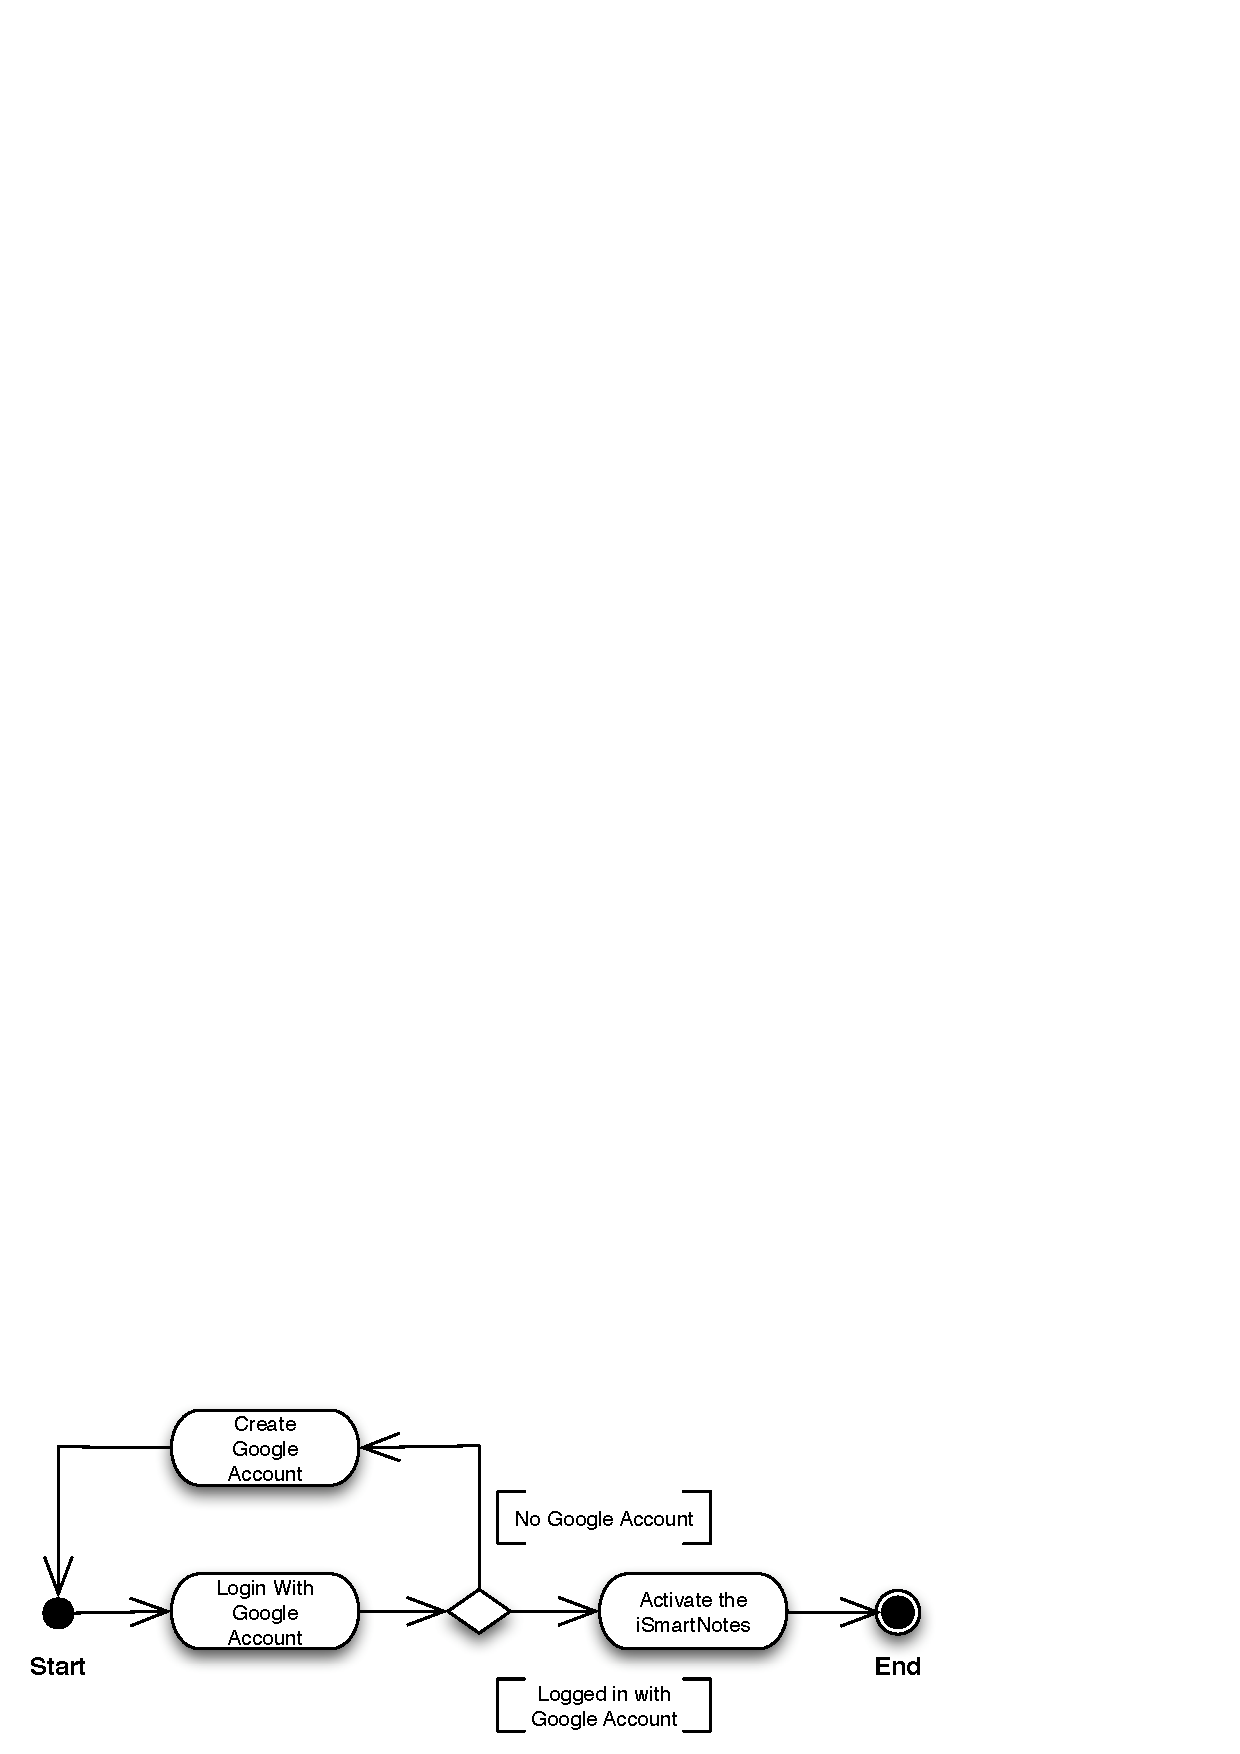
\includegraphics[scale=0.6]{charts/activate_iSmartNotes.png}
\caption{The iSmartNotes application activation with the Google Account.}
\label{fig:ismartnotes_activation}
\end{center}
\end{figure}
The skim of functionality offered by iSmartNotes is demonstrated on figure~\ref{fig:workon_ismartnotes}.
\begin{figure}[ht]
\begin{center}
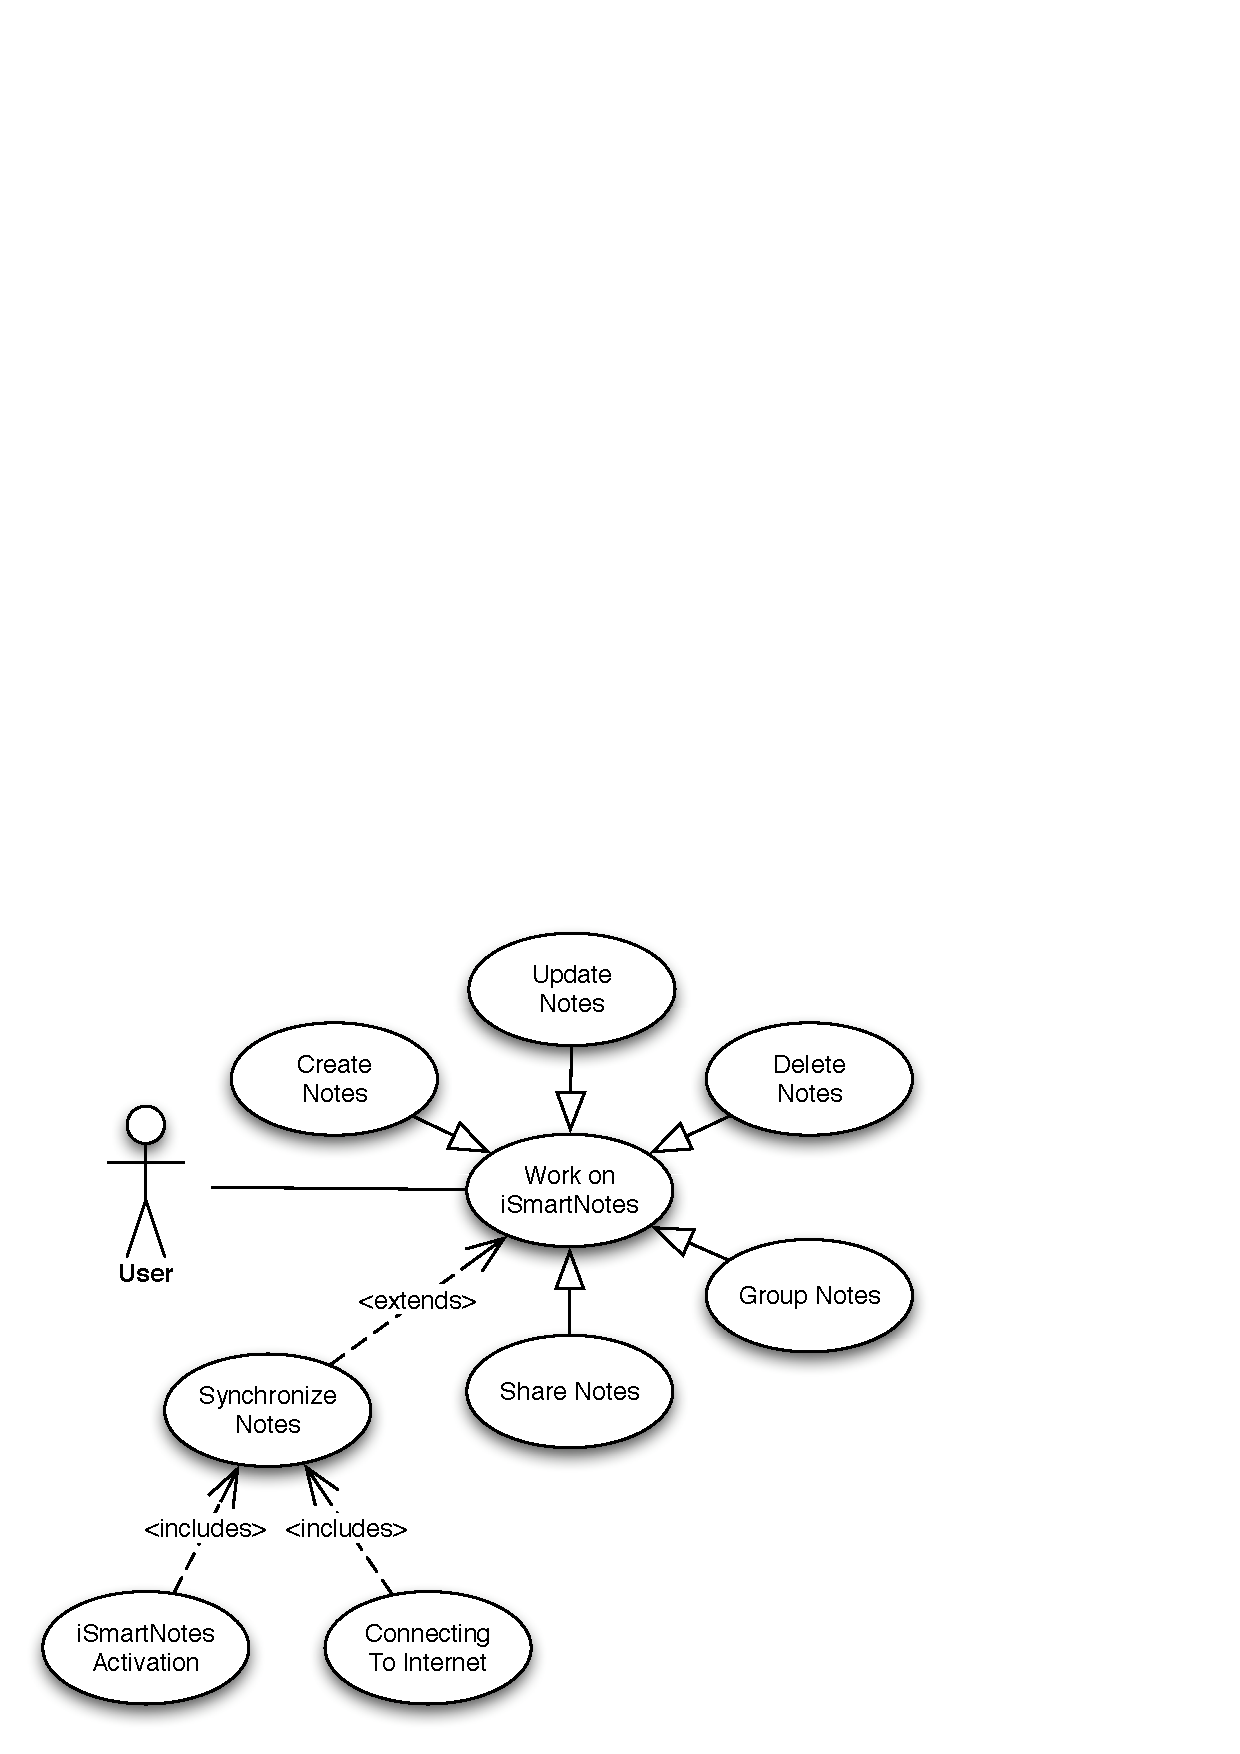
\includegraphics[scale=0.5]{charts/work_on_iSmartNotes.png}
\caption{The iSmartNotes application use cases.}
\label{fig:workon_ismartnotes}
\end{center}
\end{figure}
This includes the CRUD operations and three extra features. The notes can be easily grouped together in named tabs. This should make organizing and finding notes much easier. Secondly it should be possible to publish the notes marked as shared. Finally the synchronization feature that requires iSmartNotes activation and network connection to contact with the web based part of SmartNotes. What needs to be discussed is the cooperation between those two parts iSmartNotes and web based part of SmartNotes. The relation between them and the functionality offered to the user and administrator are shown on figure~\ref{fig:ismartnotes_smartnotes}. 
\begin{figure}[ht]
\begin{center}
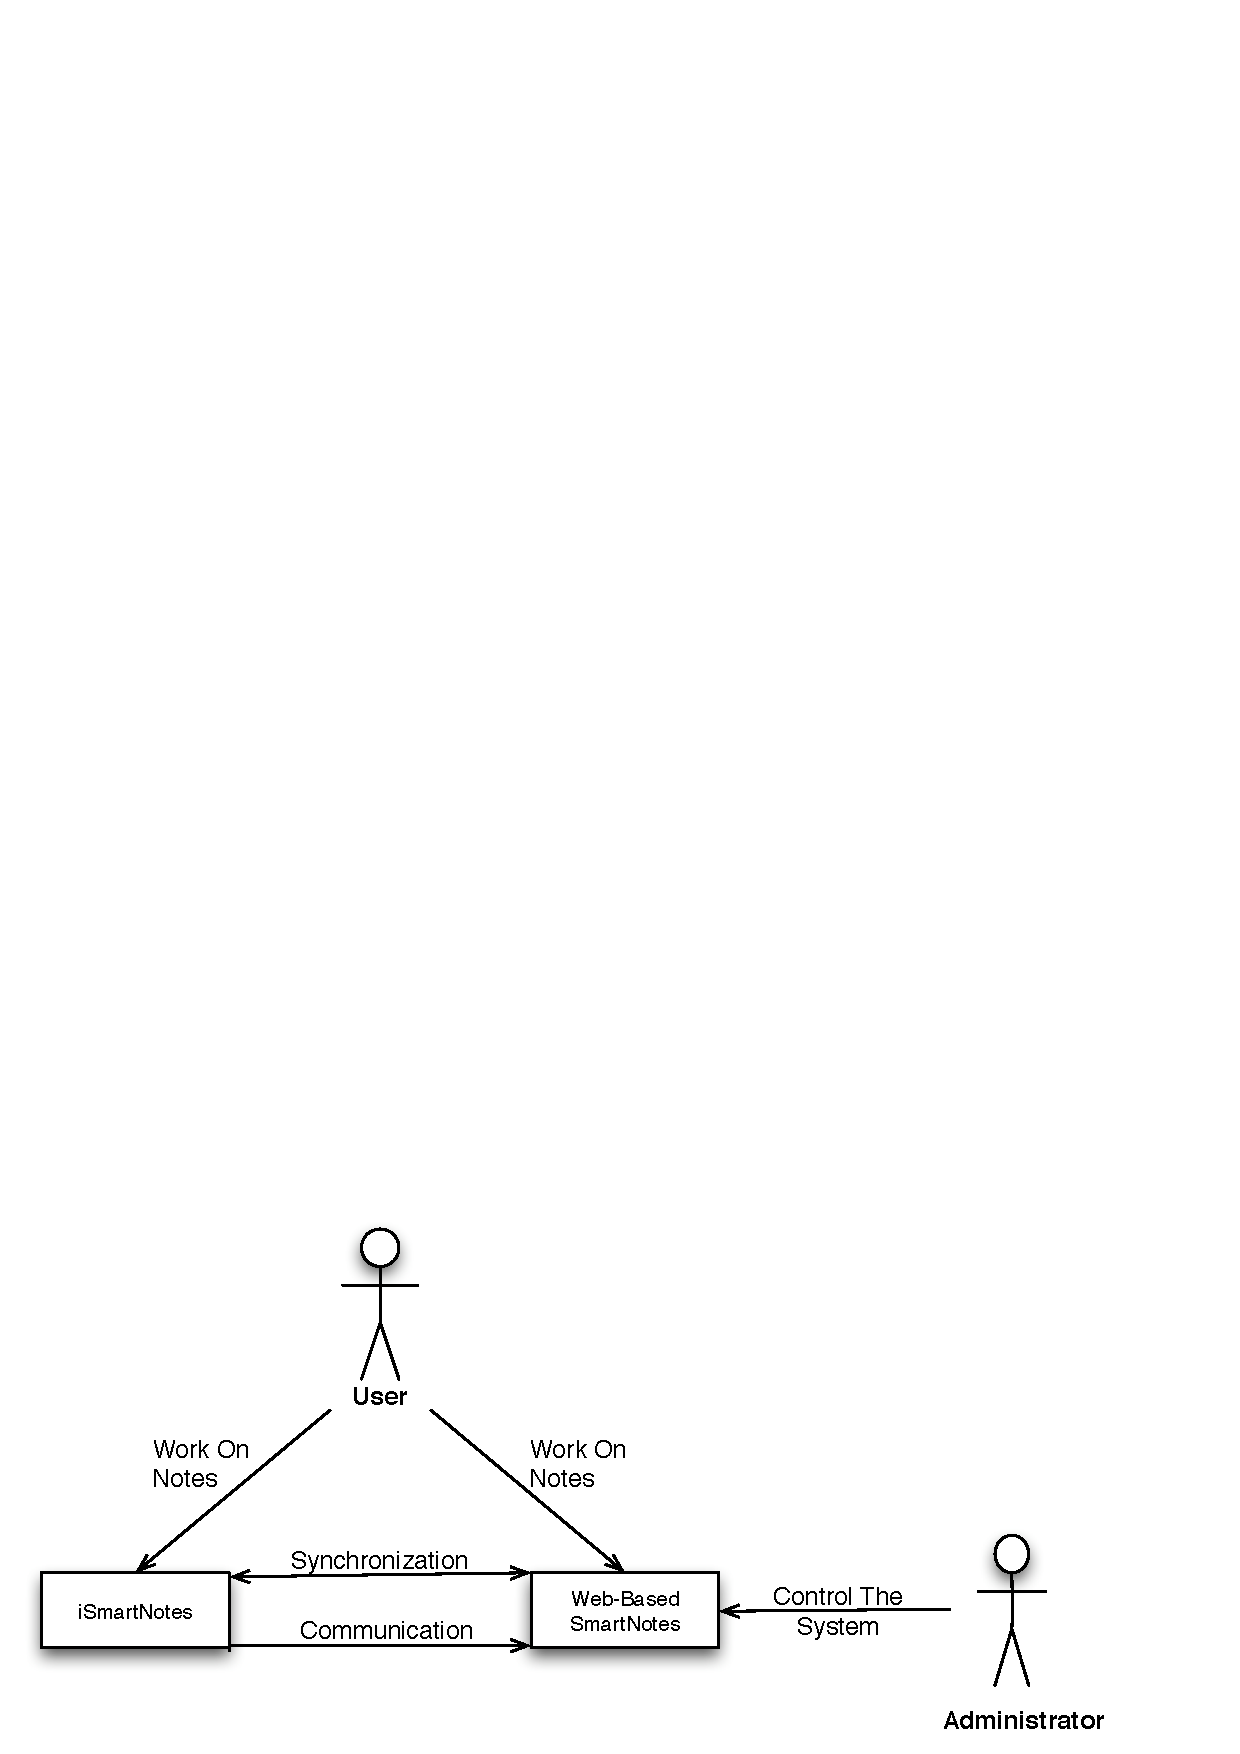
\includegraphics[scale=0.5]{charts/iSmartNotes_SmartNotes.png}
\caption{The cooperation of iSmartNotes and web based SmartNotes.}
\label{fig:ismartnotes_smartnotes}
\end{center}
\end{figure}

It is interesting concept to allow the user work on iSmartNotes and on the Web based part of SmartNotes exchangeably  and letting the SmartNotes application care for work synchronization. This was also marked on the discussed picture. However that is a remark of what could be done to make the application more functional and elastic but the user functionality of the web interface of realized project will be mineralized. On the Other hand administrator will get the access to such a tools like datastore data browser, system status or application dashboard described in section~\ref{sec:gae_general}. This can help to fast diagnose that something is going not right with the application and rollback it to the latest stable version. Moreover  it can indicate that the rescuers are not sufficient to serve the traffic and eventually extend them. Those tools work great with cooperation with Google Webmaster Tools and the Google Analytics as they can provide more information concerning the web page and its visitors.

Some additional explanations requires the synchronization feature. It will be realized by the version control system which were introduced in section~\ref{sec:popular_vcs}. No matter if the user works online or not he will have the full access to his notes and when he can use Internet notes can become synchronized. As marked on the graph from figure~\ref{fig:ismartnotes_smartnotes} the synchronization process is bidirectional from the web based part of SmartNotes which plays a role of main server and the iSmartNotes playnig the role of clients and reverse. That should allow to update the notes which could be for example edited just before leaving the office or push the just added list of things to do after coming from vacation. Next thing marked on the graph from figure~\ref{fig:ismartnotes_smartnotes} is the one directional communication between iSmartNotes and SmartNotes which should be understand as a additional logic allowing the to perform some operations on the user side by the help of iSmartNotes. That should include displaying the user information's about some important events like availability of new feature or information about availability of newer version.  Its one directional as it will be iSmartNotes application which will be in order to get this informations from the SmartNotes server and display it to the user. The presented functionality definitely does not fully exploit the possible feature list but as mentioned in section~\ref{subsec:vcs_comparison} it is a good practice to keep the application as simple as possible and focus on a set of clearly defined key features.
\section{Functional description}\label{sec:functional_descr}
The SmartNotes application should run on a infrastructure that can ensure high availability and be ready to handle high load. Assuring easy system maintenance and availability for future expanding wold be also strongly desirable features. It is not pointless to mention that all this features use resources what means that financial model is really on importance. That are is developer 10,000-foot view for the system requirements.
Users should get well informed about it, what it does and shout be able to easily start to use SmartNotes. For this reason the landing page should be informal with and support make it easy to get started. It would be best it it wold be international to reach greater group of users.

From the architectural point of view SmartNotes is though as a simple client-server application. The only one small difference is that the SmartNotes application uses DVCS which makes all the machines access same set of commands and make their hard disks hold the entire repository with it history. It may be confusing that it still remains a client-server architecture. In dead it is a little strange but just like centralized VCS don't know any other architecture than client-server the distributed version control use it as one of possible use cases. In that case one of the machines fulfills a role of reverential server to which all remaining machines direct its requests. It is a kind of public repository that holds most recent version.

 % System concept
\chapter{System Description}\label{chap:description}
\section{Google App Engine platform}\label{sec:gae}
\section{Mercurial on Google App Engine}\label{sec:hg_on_gae}
\section{Cacoa interface}\label{sec:cacoa}  % System description
\chapter{System Description}\label{chap:sys_description}
The present chapter covers the system design including specific solutions that have been chosen for the realization of the SmartNotes application. The system concept, introduced in Chapter~\ref{chap:concept}, will become extended by describing certain elements of implementation and problems found during the development process. This should allow the reader have a deeper view into the SmartNotes application including functions that it offers and platform that it runs on.
\section{Google App Engine platform}\label{sec:gae}
Google App Engine seems to be an outstanding development platform. For all the reasons mentioned in~\ref{sec:gae_general}, it has been decided to be used as the main platform for SmartNotes before any other hosting services. Besides, GAE appears to be highly competitive in terms of cost calculations, which are described in Section~\ref{subsec:gae_calculations}. After registering the application with a unique name, it can be easily uploaded to Google and after a few seconds it is accessible to its users.

As stressed in Section~\ref{subsec:sync_scenarios}, synchronization scenarios use the client-server architecture. When running on GAE platform which is, as mentioned in~\ref{sec:gae_general}, a distributed vault-tolerant infrastructure where two subsequent request may be served by different machines located in separate data centres. Thus from the addressing scope the application can still be treated as a centralized server. In case the application requires state awareness it is the developer's role to make it so. Otherwise, the fact that the application is served from multiple machines is completely transparent from the functional point of view.

SmartNotes uses only some of the components supported by GAE and t he ones which make a part of SmartNotes application with relation with other third-party elements are presented in Figure~\ref{fig:smartnotes_components}. This is especially important as it presents all the application top level components together with marked interfaces between the particular functional blocks. This particular diagram strongly corresponds with the diagram from Figure~\ref{fig:ismartnotes_smartnotes}, which in a more general way presents the cooperation of SmartNotes and iSmartNotes with differentiated roles of the administrator and the user. 

The most complicated structure is the SmartNotes component, which is marked as an individual system. It does not require the iSmartNotes to realize its functionality. For this reason, the SmartNotes component could work with any kind of client application using the interface that the tool provides, or the interface of Mercurial HTTP chains of requests and responses that needed a back-end redesign to accommodate conditions set by GAE. The issues connected with the cooperation of Mercurial and GAE are the topic of Section~\ref{sec:hg_on_gae}. 

Furthermore, SmartNotes uses three additional interfaces which are used to interconnect the Google App Engine component with Mercurial adopted to run on GAE as well as separately, admin and user interfaces provided by SmartNotes. Each of the three components is connected in a different way. Whereas the webapp framework has a low Python overhead as mentioned in Section~\ref{subsec:webapp} and was chosen to serve the connection between the Mercurial and the Google App Engine componet, for performance reasons, it is Django which is the best choice when it comes to building nontrivial web-based functionality for reasons mentioned in Section~\ref{subsec:django}. The remaining two elements used by the GAE subsystem are the Google Account and the Datastore. The role of the first one has been presente in detail while discussing the iSmartNotes activation process in Section~\ref{subsec:ismartnotes_activation}. Some of the Datastore details will be covered in Section~\ref{sec:hg_on_gae}. 
\begin{figure}[ht]
\begin{center}
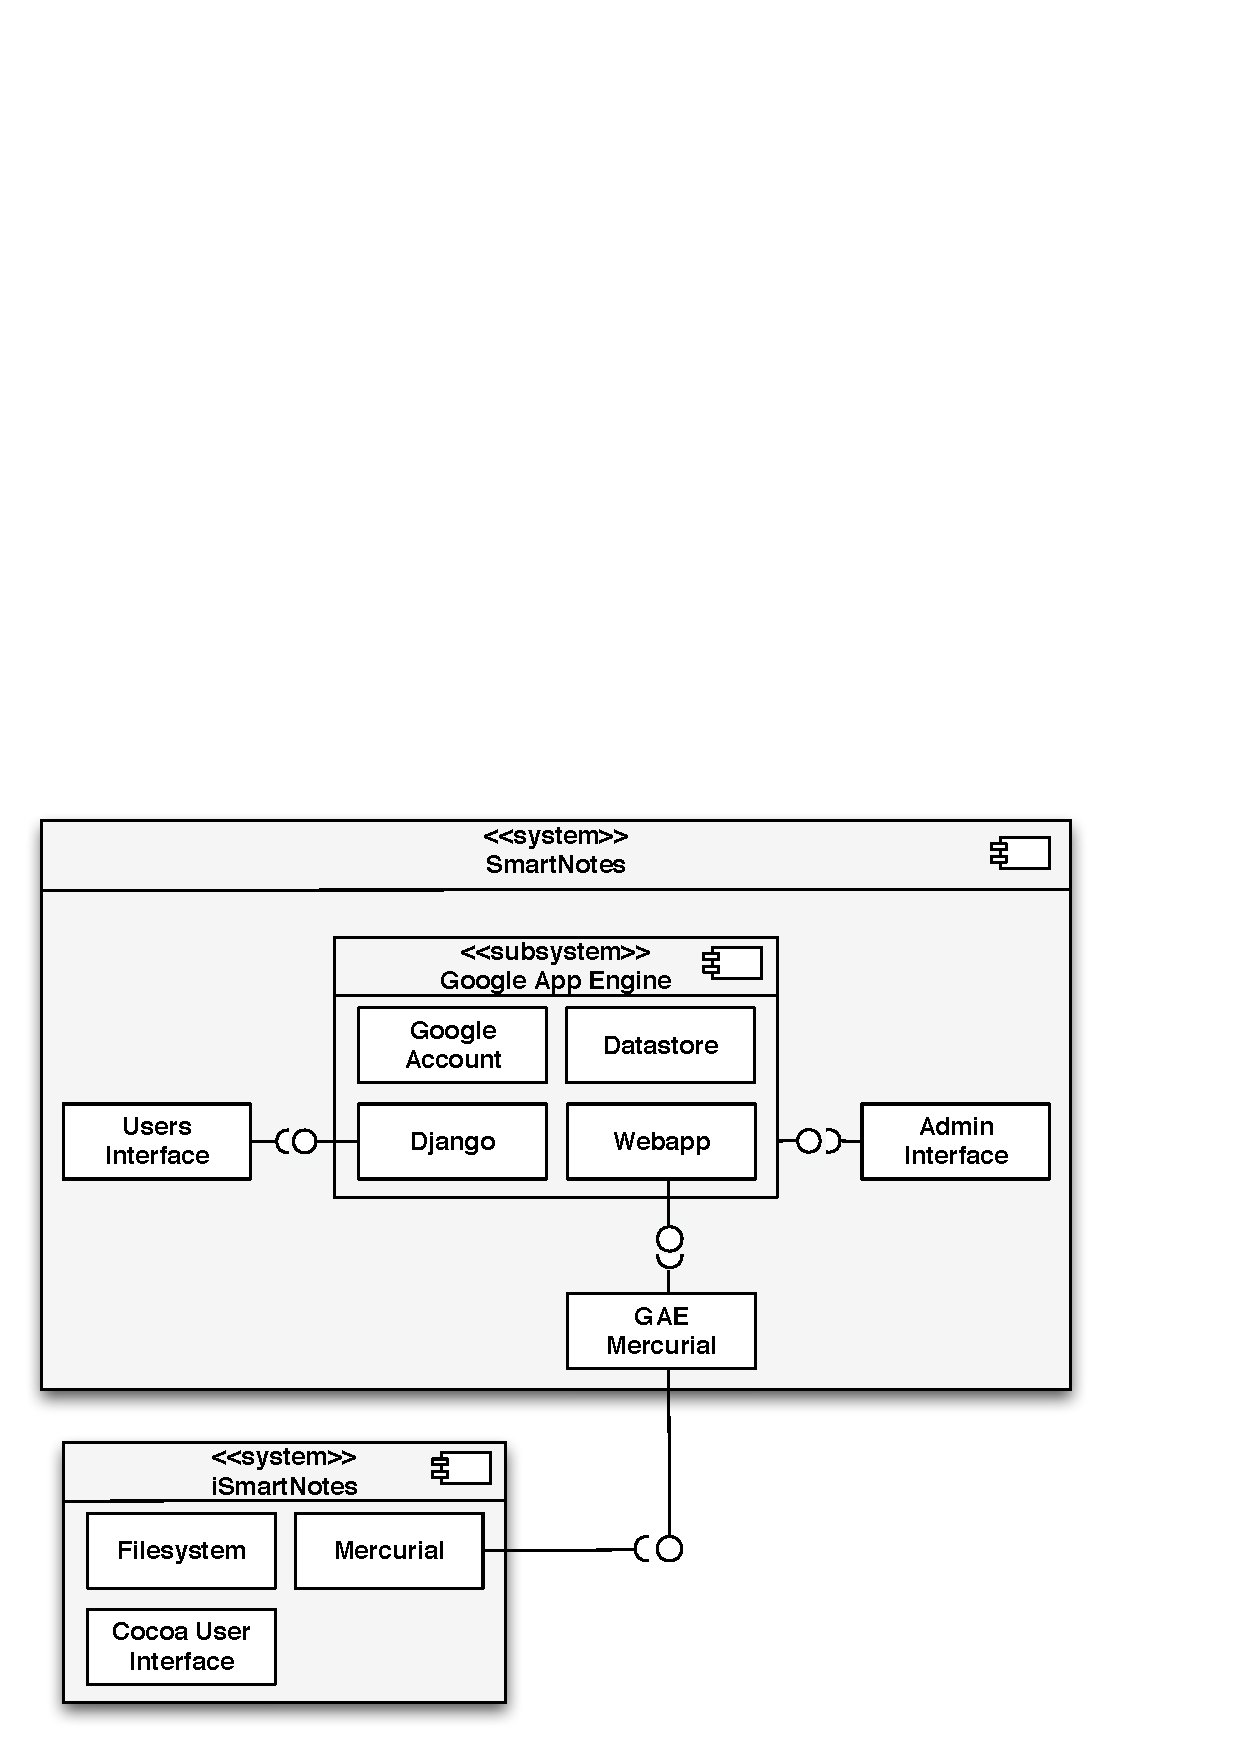
\includegraphics[scale=0.6]{charts/smartnotes_componets.png}
\caption{The components diagram of  the SmartNotes application with marked interfaces between the functional blocks.}
\label{fig:smartnotes_components}
\end{center}
\end{figure}

The second independent system is the iSmartNotes component, which remains independent until the user decides to activate it to use the synchronization feature. For this purpose, it requires a Mercurial server to interact with. The iSmartNotes, as presented in Figure~\ref{fig:smartnotes_components}, is build with three components. Firstly, the file system of the client's operating system which is the classical space where VCSs allocate their repositories. Secondly, Mercurial VCS which on the client site does not require any modifications. Finally, the Cocoa user interface whose presentation is provided in Section~\ref{sec:cocoa}.

\subsection{Financial calculations}\label{subsec:gae_calculations}
\section{Mercurial on Google App Engine}\label{sec:hg_on_gae}
\section{Cocoa user interface}\label{sec:cocoa} % System evalualtion
\chapter{System Evaluation}\label{chap:eval}
One of the aims stated for this study, as listed in the Chapter~\ref{sec:Introduction}, was to write a Python application with scalability in mind. Therefore, this chapter is devoted to presenting a thousand-feet view of the application so that the implementation described in former chapters could be taken as only one of the many possibilities to realise the intended system characteristics as well as functionality. The second section of the chapter presents a discussion of SmartNotes application metrics gathered using benchmarking tools such as \texttt{autobench} or \texttt{siege} and statistics from the Google App Engine dashboard. The present chapter, together with Chaper~\ref{cha:conclusions}, also summarises the results of the subject of this study. 
 
\section{Presentation of the final result}\label{sec:result}
Apart from a client-server architecture whose segments were presented in Figure~\ref{fig:smartnotes_components}, SmartNotes has the features of flexibility, scalability and security described in Section~\ref{sec:gae}. The web interface of the application is a simple, internationalized one that provides general information about the project and allows the iterated users access its functionality. Currently, the latter involves merely creating a SmatNotes account by using the Google Account as described in Section~\ref{subsec:ismartnotes_activation} and later receiving an activation key, the process being straightforward as presented in Figure~\ref{fig:sn_web_interface}. Finally, the users pass the activation code to the iSmartNotes application in order to take the advantage of synchronization feature allowing the users, as described in Section~\ref{sec:functionality_descr}, to work on their notes and perform synchronization whenever they may wish. The main iSmartNotes window is presented in Figure~\ref{fig:ismartnotes_window}; specifically, it has a simple text area where notes can be edited, and a \texttt{Sync} button that, depending on network connectivity, will perform synchronization on the local machine or additionally using the SmartNotes network infrastructure. This basic attempt realises the functionality, excluding sharing and grouping notes which are extensions to the present functionality and will be added to the SmartNotes application beyond the focus and implementation completed in this study. It can be clearly noted that the tool cannot compete with such applications like the ones introduced in Section~\ref{sec:popular_apps}. Yet, the related work was used as a inspiration for creating a scalable foundation that could be later become more complex by adding additional functionality, hence making the gathered experience further expanded and rendering SmartNotes more attractive to users. Finally, the SmartNotes blog, feedback form and hosting the source code on a well known Open Source service does not only point to gather users’ attention, but also to find developers who find the idea interesting and collaborate on it. 
 
Technologies chosen here provide a well documented and truly active environment with a relatively low access barrier allowing direct involvement in a short time. Some of the chosen solutions, like Django or Mercurial, could become substituted with their equivalents among different language environments or using the Java language as a universal binding for the tools\footnote{Java programming language is wide know for its dynamic curve of development and impressing thread management. These features are few on the list of characteristics motivating the existence of such projects as JRuby, Jython or Quercus which are Java implementations of respectively Ruby, Python and PHP languages. That way, different runtimes can be used in one common environment, taking advantage of all of Java’s features.}.       
\begin{figure}[ht]
  \begin{center}
    \subfigure[\textbf{SmartNotes homepage with basic information and authentication}.]{\label{fig:sm_main}\includegraphics[scale=0.5]{img/SNmain_page.png}}
    \subfigure[\textbf{Authentication using the Google account}.]{\label{fig:sm_signin}\includegraphics[scale=0.24]{img/SN_signin.png}}
    \subfigure[\textbf{Obtaining the SmartNotes activation key}.]{\label{fig:sm_getSNkey}\includegraphics[scale=0.24]{img/SNget_activation_key.png}}
  \end{center}
  \caption{The view on the public web-based SmartNotes interface with basic information regarding the project and authentication.}
  \label{fig:sn_web_interface}
\end{figure}
That direction of development appears to be gathering popularity and is worth attention. However, the chosen set of components including:
 \begin{itemize}
        \item{Google App Engine -- as a platform providing scalable infrastructure and additional useful API's for mailing, imaging or remote task queues.}
        \item{Django famework -- one of Python web frameworks which attracts more and more developers trough its clean architecture, out-of-the-box usability and strong community.}
        \item{Mercurial -- pure Python version control system with a well-designed support for HTTP protocol and a zero cost of administration.}
 \end{itemize} 
is remains significantly powerful, allowing to carry out the desired functionality with easiness for further development, an aspect that should be always recalled during any design process or when choosing between concurrent solutions. That, combined with system streamlining for concrete use cases, determines why the entire system concept is highly desirable when building scalable systems.
        
\begin{figure}[ht]
\begin{center}
\includegraphics[scale=0.5]{img/SN_ismartnotes_window.pdf}
\caption{The view on the iSmartNotes application window.}
\label{fig:ismartnotes_window}
\end{center}
\end{figure}
% gae_best_practises_plus_load_tests
\section{Performance tests}\label{sec:performance}
Performance testing form does strongly depend on the research scope. Testing the application performance is only a general name for the process that should become narrowed to a single parameter or set of well defined properties. The usage of wright tool does also matter just as making appropriate assumptions and choosing wright model used as otherwise measured values could not match the real application characteristics.   

The analyses done in this chapter are fallowing the guidelines as defined in~\cite{gae_best_practises_plus_load_tests} for testing applications that use Google App Engine:
\begin{itemize}
	\item{Use production system. Most of web frameworks provide a development including sever that can be easily run on the local machine. What speedups the development at one side cant be used for production purposes. This environment divers significantly from the deployment system and cant be to give much information of final system performance.}
	\item{Gradual ramp up. The goal of load tests is to probe the system reaction for a certain input parameter sets. Therefore its strongly desirable to make it remind the realistic cases. Besides the resources of Google App Engine are granted only when the application needs them. That motivates a wrap up just before the wright test takes place.}
	\item{Realistic load. Is seams pointless to run test for a situation that the system is unlikely to reach.}
\end{itemize}
The fallowing part of this subsection presents a graphical illustration for selected performance metrics of SmartNotes application running on Google App Engine. Taking into account the parameters such as the rate of opened connections and reached request rate the analyses in the first step will focus on the variations of the response rate and will be finalised with a comparison of the average response time between different techniques. This includes a internalized dynamic content, cached page and same page served as static content. The first is a most classical case when some parts of page depending on state may differ, second one makes use of highly popular caching technique and lastly the special infrastructure devoted only for serving static content. All of these will become wider dissed by analysing corresponding results. 

The view on dashboard of SmartNotes application shown in Figure~\ref{fig:sn_dash_view} exposes a plot of request rate timeline for two different scenarios. The first  one marked as~\textit{(a)} illustrates a regular usage case with none anomalies wheres the second figure~\textit{(b)} presents a case when outgoing bandwidth became exceeded. This is most basic way of tracking the application performance and status. Providing couple of other tools which were discussed in Section~\ref{sec:gae_general} admin interface is truly functional yet easy to use. Providing a logs browser it leaves a place where user can place his application specific informations on several logging levels.     
\begin{figure}[ht]
  \begin{center}
    \subfigure[\textbf{Regular situation with average of about one\newline request per second}.]{\label{fig:dash_normal}\includegraphics[scale=0.18]{img/DASH_Regular_stats.png}}
    \subfigure[\textbf{Application reaching the outgoing bandwidth limit on heavy traffic situation with the maximum of 170 requests per second}.]{\label{fig:dash_out_of_bandwith}\includegraphics[scale=0.2]{img/DASH_Out_of_bandwith.png}}
  \end{center}
  \caption{The view on the public web-based SmartNotes interface with basic information regarding the project and authentication.}
  \label{fig:sn_dash_view}
\end{figure}
The system of quotas of introduced by Google provides to phase limitations the daily limits and narrowed most common to minute quotas.The second one is a protection for load high peaks or any malicious or testing software that without it could let to letting the target application out of resource in just a couple of minutes. Thats exactly the case uncounted during the tests by receiving responses with \texttt{503 Service Unavailable} status codes when crossing the short tame quota and \texttt{403 Forbidden} responses after running over the daily limits.

The author has chosen Open Source tools like \texttt{httperf} from HP and \texttt{autobench} wrapper to carry out the tests for the main SmartNotes web page. This tools were chosen beyond others researched\footnote{That list includes tools like \texttt{siege} and \texttt{ab} which are popular Open source load testing programs.} due support for a gradual increase of connection rate and extended output. Each of the tests which results are presented in Figures~\ref{fig:sm_benchmark_normal}, \ref{fig:sm_benchmark_cache}, \ref{fig:sm_benchmark_static} and \ref{fig:sm_resp_time_comapre} uses the same set of input parameters:
\begin{itemize}
	\item{500 connections per test. This connected with twenty second connection timeout allowed to reach up to 400 concurrent connections.  }
	\item{3 requests per connection. This implies a total number of 1500 requests per test. This parameter was chosen with respect to the short term quota limit of $7, 400$ requests per minute.}
	\item{Generated connection rate stared at 25 connections per second and by each test was gradually increased by factor of 10 up to reaching the rate of 145 connections per second. That allowed to make 12 tests for in each of test series.}
	\item{Each of tests is identified using multiplication of generated connection rate and number of request per second as the horizontal axis labels. That values correspond to the theoretical request rate or the client-side request rate.}
\end{itemize}

First of techniques that was tested was a classical dynamic page which was using the system resources to determine the language and present internationalized content. For grater flexibility and minimising the repetitions of common parts author decided to use template inheritance. This in basic let to use template blocks in a way remaining the object oriented  programming. However both of them cost the CPU time and in a case of high rated page seam not to be the most suitable solution. The most common approaches to this problem are presented by next two techniques: using cache or serving as static content. The most interesting part is to observe the differences in serving the same content using each of those techniques. One of parameters that has a great impact on the  rest is the server-side connection rate that in Figures~\ref{fig:sm_benchmark_normal}, \ref{fig:sm_benchmark_cache} and \ref{fig:sm_benchmark_static} was presented using green lines. I case of dynamic page the average connection rate become saturated around 45 connection per second what gives the request rate of 135 requests per second. 
\begin{figure}[ht]
  \begin{center}
	\includegraphics[scale=0.4]{charts/benchmarks/normal4.pdf}
  \end{center}
  \caption{Response rate statistics for dynamic page served using the Django framework.}
	\label{fig:sm_benchmark_normal}
\end{figure}
This number is close to the mentioned before short time limit of $7, 400$ requests per minute. The test were done several times that way to as close as possible to the this quota limits watching to receive replies with the \texttt{200 OK} response code. Additionally it is also interesting the observe the distribution of the minimum, average and maximum response rate with increasing value of average request rate. In ideal case all of this four factors would fallow identical linear curve.     

The second technique is cashing. It is a solution bundled into many web frameworks including Django which as noted  in Section~\ref{sec:gae_general} is supported by GAE. Concept of this technique is based on storing data in some fast accessible space called cache and with the help of it repeating calls can shorting the request path. A simple usage of cashing system could look as presented in Listing~\ref{code:py_cache}. The function \texttt{get\_from\_cache} returns the data calculated by function called \texttt{some\_time\_consuming\_calculations} that next becomes located into control of \texttt{memcache}\footnote{Memcached is a distributed, memory based cashing system. This only one of possible caching backends such like file-cache or database based storage engines however it is mostly used for its speed and support for multi-machine work mode.} for a time defined by the \texttt{expire\_time} variable. In case a subsequent calls coming before one hour from the first calculation of \texttt{data} they wont call the \texttt{some\_time\_consuming\_calculations} function but return the value stored by the \texttt{key} name.        
\lstset{language=Python,caption=Simple cache usage example in Python.,label=code:py_cache,
basicstyle=\scriptsize,         % the size of the fonts that are used for the code
showspaces=false,               % show spaces adding particular underscores
showstringspaces=false,         % underline spaces within strings
showtabs=false,                 % show tabs within strings adding particular underscores
tabsize=2,                    % sets default tabsize to 2 spaces
captionpos=b,                   % sets the caption-position to bottom
breaklines=true,                % sets automatic line breaking
breakatwhitespace=false,        % sets if automatic breaks should only happen at whitespace
escapeinside={\%*}{*)}          % if you want to add a comment within your code
}
\lstinputlisting{src/samples/py_cache.py}
When the \texttt{some\_time\_consuming\_calculations} is truly resource consuming this technique can bring efficient savings. In case test results for cached version of page the plot from Figure~\ref{fig:sm_benchmark_cache} does only slightly differ from the curves of the dynamic version from Figure~\ref{fig:sm_benchmark_normal}. Used HTTP headers shown in Listing~\ref{code:resp_headers} can help to avoid subsequent calls from a single user by using his browser-cache mechanisms.The test client was ignoring them as it was supposed to test the worst case scenario when all of the connections being opened come from different users that use browsers ignoring the cache specific headers including \texttt{Expires}, \texttt{Vary}, \texttt{Last\-Modified}, \texttt{ETag} and \texttt{Cache\-Control}. 
\lstset{language=HTML,caption=Server response headers for cached content.,label=code:resp_headers,
basicstyle=\scriptsize,         % the size of the fonts that are used for the code
showspaces=false,               % show spaces adding particular underscores
showstringspaces=false,         % underline spaces within strings
showtabs=false,                 % show tabs within strings adding particular underscores
tabsize=2,                    % sets default tabsize to 2 spaces
captionpos=b,                   % sets the caption-position to bottom
breaklines=true,                % sets automatic line breaking
breakatwhitespace=false,        % sets if automatic breaks should only happen at whitespace
escapeinside={\%*}{*)}          % if you want to add a comment within your code
}
\lstinputlisting{src/samples/headers_cache.txt}

On the other hand it does not mean that that using caching did not bring anything. Because the requests to cache are normally much cheaper from the requests that involve the server-side operations the binding quota limits are lower and allow for $8,640,000$ API calls a day. Usage of \texttt{memcached} did help to reduce the CPU usage what is a big advantage of this technique. However it should be taken into account that usage of memory caching will consume additional memory, make the system little more complex and by itself isn't a fault tolerant storage. Besides one of the biggest problems regarding cache is expiring it content. In case some page component changed on some of pages the easiest way is to flush all the cache content. In case of application that profile has similar number of read as write operations cache will be much harder to implement. This solution suits best applications of high read rate.      
\begin{figure}[ht]
  \begin{center}
	\includegraphics[scale=0.4]{charts/benchmarks/cache4.pdf}
  \end{center}
  \caption{Response rate statistics for cached page. Realised using the Google memcache API.}
  \label{fig:sm_benchmark_cache}
\end{figure}

The last tested approach was to serve the entire page as a static content. It should be noted that the infrastructure used for this purpose differs strongly from the application server. It takes the advantage of storing stateless content and minimum server overhead. The implementation details belong to the Google company however the they exist Open Source projects like \texttt{lighttpd} or \texttt{nginx} which share the same idea. Those differences can be easy observed in Figure~\ref{fig:sm_benchmark_static}. Until reaching the level of 235 requests per second the response rate curve was fallowing the server-side request rate curve with low value variation not crossing the factor of $5 \%$ of average value. In this case the CPU usage rate was even lower than using caching and did not require any additional memory usage like in case of \texttt{memcached}. It should be requires much more work to be integrated with the application replacing it prior dynamic content. That task might be sometimes even impossible to be done result in bed final experience when done not wright. Thus it definitely is interesting option for applications that are stateless or use lots of different media files.             
 \begin{figure}[ht]
  \begin{center}
	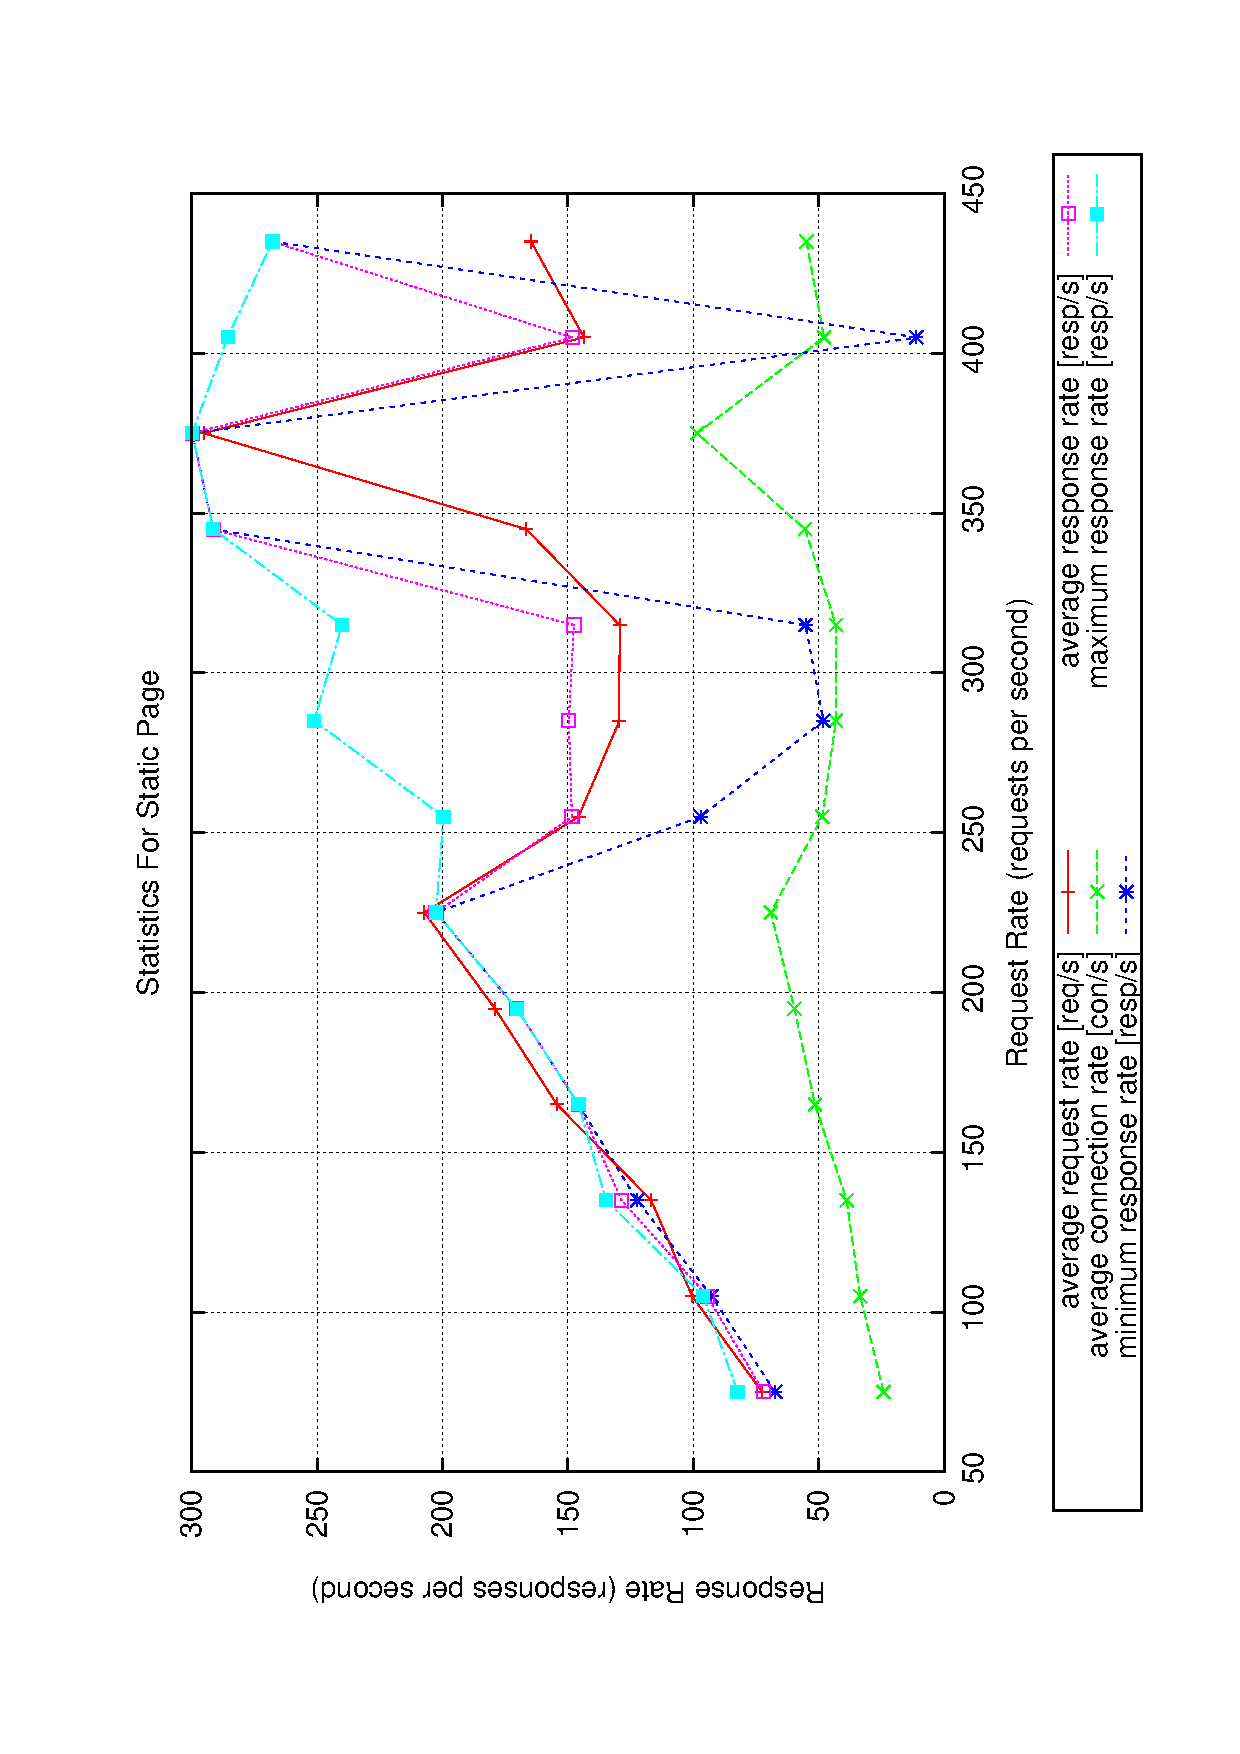
\includegraphics[scale=0.4]{charts/benchmarks/static4.pdf}
  \end{center}
  \caption{Response rate statistics for static page with use of static content server.}
\label{fig:sm_benchmark_static}
\end{figure}

An interesting comparison presented in Figure~\ref{fig:sm_resp_time_comapre} which collates various techniques used together by focusing on the average response time. It is one of the parameters that has a huge inpact on the user experience    
\begin{figure}[ht]
  \begin{center}
	\includegraphics[scale=0.4]{charts/benchmarks/final4.pdf}
  \end{center}
  \caption{Comparison of average response times among various cases including serving dynamic content, caching response in memory or making use of static content server.}
	\label{fig:sm_resp_time_comapre}
\end{figure}   % Conclusion
     
		       %% Honors theses are required to 
                          %% have an unnumbered chapter
                          %% for conclusions.  The file
                          %% Conclusion.tex should begin
                          %%   
                          %% \chapter*{Conclusion}
                          %% followed by the appropriate
                          %% text.
\begin{spacing}{1.0}
	\bibliographystyle{plain}
	\bibliography{mbib}
\end{spacing}

%\include{biblio}            %% Calls biblio.tex.  See below.
%-->\Appendix                 %% Use this command if you have one 
                          %% appendix. Use \Appendices if you 
                          %% have more than one.
	
%-->\include{toolong}         %% Calls toolong.tex which contains
                          %% an appendix.

\end{document}